
\begin{appendices}
	
	\section{Разработен числен код}

В това допълнение ще представим разработеният за дисертационният труд числен код Mjølnir\footnote{Сорс кодът може да бъде намерен на https://github.com/ValentinDeliyski/Mjolnir\_GRRT}. Неговата главна цел е следната: \\

\emph{Да интегрира уравненията за движение на изотропните геодезични линии в произволно статично и аксиално симетрично пространство - време (Б.1а - Б.1б), като към тях зацепи  уравнението за паралелен пренос на вектора на поляризацията в това пространство (Б.1в) и уравнението за поляризиран лъчист пренос през произволна излъчваща среда (Б.1г):}

\begin{subequations}
	\begin{equation}
		\frac{dx^\mu}{d\lambda} = \frac{\partial H}{\partial k_\mu}
	\end{equation}
	\begin{equation}
		\frac{d k_\mu}{d\lambda} = - \frac{\partial H}{\partial x^\mu}
	\end{equation}
	\begin{equation}
		k^\nu\nabla_\nu f^\mu = 0
	\end{equation}
	\begin{equation}
		\frac{d}{d\lambda} \begin{pmatrix}
			\mathcal{I}_\nu\\
			\mathcal{Q}_\nu\\
			\mathcal{U}_\nu\\
			\mathcal{V}_\nu
		\end{pmatrix} = 
		\begin{pmatrix}
			\mathcal{J}_\mathcal{I,\nu}\\
			\mathcal{J}_\mathcal{Q,\nu}\\
			\mathcal{J}_\mathcal{U,\nu}\\
			\mathcal{J}_\mathcal{V,\nu}
		\end{pmatrix}
		-	\begin{pmatrix*}[r]
			\kappa_\mathcal{I,\nu} & \kappa_\mathcal{Q,\nu} & \kappa_\mathcal{U,\nu} & \kappa_\mathcal{V,\nu}\\
			\kappa_\mathcal{Q,\nu}& \kappa_\mathcal{I,\nu}& -\rho_\mathcal{U,\nu}& \rho_\mathcal{V,\nu}\\     	
			\kappa_\mathcal{U,\nu}& -\rho_\mathcal{V,\nu}& \kappa_\mathcal{I,\nu}& \rho_\mathcal{Q,\nu}\\	  
			\kappa_\mathcal{V,\nu}& \rho_\mathcal{U,\nu}& -\rho_\mathcal{Q,\nu}& \kappa_\mathcal{I,\nu}\\
		\end{pmatrix*}
		\begin{pmatrix}
			\mathcal{I}_\nu\\
			\mathcal{Q}_\nu\\
			\mathcal{U}_\nu\\
			\mathcal{V}_\nu
		\end{pmatrix}.
	\end{equation}
\end{subequations}

С негова помощ, генерирането на релативистките образи, представени на фигури (6.17, 6.18, 6.19, 8.1, 8.2 и 8.11) се случва по следният начин: Фиксира се наблюдател в точката $\vec{r}_\text{obs}$, дефиниран посредством ортонормиран базис $\{e^\mu_{(t)},e^\mu_{(r)},e^\mu_{(\theta)},e^\mu_{(\phi)}\}$, за който се определя зрително поле върху небесната му сфера $\mathcal{Z}$, посредством ъглите $\{\alpha,\beta\}$ (виж допълнение В). Това зрително поле се разглежда като съвкупност от пиксели, всеки от който съответства на дадени $\{\alpha_i,\beta_i\}$. Използвайки изразите (В.5):
\begin{subequations}
	\begin{equation}
		L_z = \sqrt{g_{\phi\phi}}\cos\beta\sin\alpha
	\end{equation}
	\begin{equation}
		E = \frac{1}{\xi}\left(1 + \gamma L_z\right),\quad \xi = \sqrt{\frac{g_{\phi\phi}}{g_{t\phi}^2 - g_{tt}g_{\phi\phi}}},\,\, \gamma = -\frac{g_{t\phi}}{g_{\phi\phi}}\xi
	\end{equation}
	\begin{equation}
		p_r = \frac{1}{E}\sqrt{g_{rr}}\cos\beta\cos\alpha\big\vert_{\vec{r} = \vec{r}_\text{obs}}
	\end{equation}
	\begin{equation}
		p_\theta = \frac{1}{E}\sqrt{g_{\theta\theta}}\sin\beta\big\vert_{\vec{r} = \vec{r}_\text{obs}}
	\end{equation}
	\begin{equation}
		p_\phi = \frac{L_z}{E},
	\end{equation}
\end{subequations}

тази съвкупност може да се превърне в набор начални условия за динамичните уравнения (Б.1а - Б.1б). Фиксирайки също и подходящи начални и гранични условия за (Б.1в) и (Б.1г), Mjølnir интегрира системата (Б.1), чието решение са функциите $\mathcal{I}_\nu(\alpha,\beta)$, $\mathcal{Q}_\nu(\alpha,\beta)$, $\mathcal{U}_\nu(\alpha,\beta)$ и $\mathcal{V}_\nu(\alpha,\beta)$ за $\{\alpha,\beta\}\in\mathcal{Z}$. В следващите подточки ще представим процедурата по решаването на системата, както и сравнение на получените образи с подобни числени програми \cite{Bronzwaer2020}, \cite{Ipole_Code}.

\subsection{Процедура по интегриране на динамичните уравнения}

Решаването на системата (Б.1) има една особеност. Началните условия за (Б.1а) и (Б.1б) се задават при наблюдателя, докато зети за (Б.1в) и (Б.1г), на безкрайност от него. Следователно интегрирането трябва да протече в два стъпки:\\

\textbf{1) Вакуумно интегриране}. В тази стъпка, Mjølnir интегрира единствено уравнения на Хамилтон (Б.1а) и (Б.1б), \emph{започвайки от наблюдателя}, в интервала $\lambda\in[0,\lambda_\text{stop}]$\footnote{Причината да интегрираме \emph{назад} по историята на лъчите е следната: Ако разгледаме елементарен излъчващ обем, без да налагаме предположения за механизъма на излъчване или термодинамичното състояние на средата, можем в общия случай да приемем, че той излъчва в целия набор пространствени ъгли $\Omega$ (дори и неравномерно). Далечен наблюдател обаче, би засякъл единствено това лъчение, идващо от областта $d\Omega$, която е свързана с него, посредством уравненията (Б.1а) и (Б.1б). Започвайки интегрирането от наблюдателя, ние автоматично избираме единствено областта $d\Omega$, която допринася към образите.} \footnote{Общият термин за интегрирането на лъчи, започващи от наблюдателя, "назад" по траекторията им, до достигане на \emph{източника}, е \emph{обратно тресиране на лъчите} (backwards ray tracing). Този тип "обратно"$\,$интегриране се използва при \emph{всички} числени програми, в които е дефиниран наблюдател, засичащ лъчението от далечен източник. То дори не е ограничено да бъде електромагнитно по характер. С подходяща смяна на Хамилтоняна в (Б.1а) и (Б.1б), процедурата по обратно тресиране на лъчите може да симулира детектирането на поток йонизиращо лъчение от масивни частици (например космичните лъчи).}, $\lambda_\text{stop} < 0$. Стойността $\lambda_\text{stop}$ се определя от динамичното състояние на дадения лъч - т.е. програмата прави проверки на всяка итерация, дали са изпълнени определени условия за прекратяване на интеграцията. Такива са например:\\

\indent \textbf{1.1)} Достигане до фиксиран, максимален брой итерации. Това подсигурява, че програмата винаги ще свърши.\\
\indent \textbf{1.2)} При наличие на хоризонт на събитията, фотони за които е изпълнено $r - r_h < \epsilon$, се приемат за попаднали върху него, и интегрирането се прекратява\footnote{Стойността за $\epsilon$, използвани в симулациите представени в този труд, е $\epsilon = 10^{-5}M$.}.\\
\indent \textbf{1.3)} Фотони за които е изпълнено $r > r_{\text{th}}$ и $p_r < 0$ са такива, които \emph{налитат към наблюдателя} от небесната сфера (т.е. от безкрайност). Следователно ако изберем $r_{\text{th}}$, така че отвъд него да няма значително излъчване от средата\footnote{Използвали сме $r_{\text{th}} = 100M$}, интегрирането може да се прекрати.\\

Друга особеност на системата (Б.1) е, че в региони, близки до гравитационният център или характерните повърхнини на пространство-времето (като хоризонта на събитията или фотонната сфера), тя става \emph{твърда}. В такъв режим, интегрирането трябва да протича с много фина стъпка $d\lambda \ll 1$. Това налага използването на \emph{адаптивен} метод за интеграция, понеже далеч от тези по региони, с оглед скорост, искаме да използваме по-груба стъпка. В Mjølnir сме имплементирали метода на Дормaнд-Принц от ред 5(4) \cite{RK45}. Той предоставя решение с точност $\mathcal{O}(d\lambda^5)$, и оценка за абсолютната $\Delta \vec{x}_\text{abs}$ и относителна $\Delta \vec{x}_\text{rel}$ грешка на всяка итерация. Тя може да се използва, заедно с алгоритъм за управление, за поддържане на оптимална стойност за $d\lambda$. Т.е. целта на това управление е поддържа възможно по-висока стойност за $d\lambda$, удовлетворявайки условията $\text{absmax} \Delta \vec{x}_\text{abs} < \delta_1$ и $\text{absmax} \Delta \vec{x}_\text{rel} < \delta_2$, за избрани от нас $\{\delta_1,\delta_2\}$. Алгоритъма за управление сме избрали на база \cite{Fekete_2022}, израз (22).\\

По време на самото интегриране, Mjølnir прави проверки за прекосяване на лъча през екваториалната равнина. Когато това стане в радиален интервал $r_\text{in} < r < r_\text{out}$, се пресмята израз (6.8) за наблюдаваният поток от модела на Новиков-Торн,. Това генерира образите от фигури (6.17) - (6.19).\\

Траекторията на лъча също така се пази в паметта на програмата, и при достигане на някое от условията 1.1) - 1.3), интегрирането на уравненията на Хамилтон (Б.1а) и (Б.1б) се прекратява. Тогава се налагат началните условия за (Б.1в) и (Б.1г) и траекторията на лъча се обхожда "напред"$,$ от $\lambda_{\text{stop}}$ до $\lambda = 0$, интегрирайки уравненията (Б.1в) и (Б.1г).

\subsection{Пресмятане на лъчистия пренос}

В момента на стартиране на пресмятането на лъчистия пренос, условията 1.1) - 1.3) са осигурили, че няма значително излъчване "назад"$\,$по лъча, и следователно налагаме началните условия:
\begin{subequations}
	\begin{equation}
		\mathcal{I}_\nu(\lambda_{\text{stop}}) = \mathcal{Q}_\nu(\lambda_{\text{stop}}) = \mathcal{U}_\nu(\lambda_{\text{stop}}) = \mathcal{V}_\nu(\lambda_{\text{stop}}) = 0
	\end{equation}
	\begin{equation}
		f^{(a)}(\lambda_{\text{stop}}) = (0,1,0,0)
	\end{equation}
\end{subequations}

Които използваме за интеграция на лъчистия пренос (Б.1в) и (Б.1г). За да направим това обаче, също е нужно да фиксираме трансформацията $f^\mu \leftrightarrow f^{(a)}$ - т.е. да дефинираме явно Стоксовия базис $\{e_{S, (t)}^{\mu}, e_{S, (K)}^{\mu}, e_{S, (\parallel)}^{\mu}, e_{S, (\perp)}^{\mu}\}$. Следвайки \cite{Bronzwaer2020} и \cite{Ipole_Code}, избираме:
\begin{subequations}
	\begin{equation}
		e^\mu_{S, (t)} = u^\mu
	\end{equation}
	\begin{equation}
		e^\mu_{S,(K)} = \frac{k^\mu}{\omega} - u^\mu
	\end{equation}
	\begin{equation}
		e^\mu_{S,(\parallel)} = \frac{b^\mu + \beta u^\mu - Ce^\mu_{(K)}}{\mathcal{N}} 
	\end{equation}
	\begin{equation}
		e^\mu_{S,(\perp)} = \frac{\epsilon^{\mu\nu\alpha\delta}u_\nu k_\alpha b_\delta}{\omega \mathcal{N}} 
	\end{equation}
	\begin{equation}
		\beta = u_\alpha b^\alpha,\,\, \omega = -k_\alpha u^\alpha,\,\, C = \frac{k_\alpha b^\alpha}{\omega} - \beta,\,\, \mathcal{N} = \sqrt{d^2 + \beta^2 - C^2},
	\end{equation}
\end{subequations}

където $b^\mu$ e вектора на магнитното поле, измерено в собствената отправна система на излъчващата плазма (със скорост $u^\mu$), и $k^\mu$ е импулса на фотона. Самата геометрия на $b^\mu$ обаче, е удобно да се задава в термини на полето $B^\mu$, измерено от статичен наблюдател със скорост $n_\mu = (1,0,0,0)$. За да намерим тази връзка, нека изразим дуалният тензор на Максуел $\tilde{F}^{\mu\nu}$ по следният начин:
\begin{equation}
	\tilde{F}^{\mu\nu} = u^\mu b^\nu - u^\nu b^\mu,
\end{equation}
и нека го проектираме върху статичният наблюдател $\tilde{F}^{\mu\nu}n_\mu = B^\nu$. Тогава можем да изразим компонентите на $b^\mu$ (използвайки факта, че $u_\mu b^\mu = 0$) чрез $B^\mu = (0, \vec{B})$, в базиса на статичният наблюдател като:

\begin{subequations}
	\begin{equation}
		b^0 = B^i u_i
	\end{equation}
	\begin{equation}
		b^i = \frac{B^i + u^ib^0}{u^0}
	\end{equation}
\end{subequations}

В числената имплементация, векторът $\vec{B}$ се използва само за задаване на геометрията на полето - т.е. той е нормиран на единица, а самата големина, измерена в отправната система на плазмата, се пресмята с израза:

\begin{equation}
	\sqrt{b^\mu b_\nu} = \sqrt{4\pi m_pc^2 \sigma n_e},
\end{equation}
където свободният параметър $\sigma$ е намагнитването на средата, $m_p$ е масата на протона и $n_e$ е концентрацията на електрони. Всички величини са пресметнати в Гаусова система единици. Удобството на така дефинираният Стоксов базис е, че в него функциите на излъчване $\mathcal{J}_{\mathcal{U},\nu}$, и тези на Фарадей $\rho_{\mathcal{U},\nu}$, се нулират.\\

Използвайки този базис, можем да трансформираме началното условие (Б.3б) от Стоксов базис към координатен (т.е. $f^\mu = e^\mu_{S, (a)}f^{(a)}$) с което да започнем интегрирането на уравнението за паралелен пренос (Б.1в). Процедурата по интегриране на лъчистия пренос тогава протича по следният начин:\\

\textbf{1)} Пропагираме вектора на поляризация в координатният базис $f^\mu$ с една стъпка, чрез уравнение (Б.1в).\\
\textbf{2)} Създаваме Стоксовия базис в сегашната точка по лъча, използвайки уравнения (Б.4а) - (Б.4д), и пресмятаме $f^{(a)} = e^{(a)}_{S,\mu} f^\mu$.\\
\textbf{3)} Пресмятаме компонентите на вектора на Стокс $\mathcal{S}_\nu = (\mathcal{I}_\nu, \mathcal{Q}_\nu, \mathcal{U}_\nu, \mathcal{V}_\nu)$, чрез изразите:

\begin{equation}
	\mathcal{S}_\nu = \begin{pmatrix}
		\mathcal{I}_\nu \\
		\mathcal{Q}_\nu \\
		\mathcal{U}_\nu \\
		\mathcal{V}_\nu
	\end{pmatrix} = 
	\begin{pmatrix}
		\mathcal{I}_\nu \\
		\mathcal{I}_{pol, \nu} \left(f^{(1)} f^{(1)*} - f^{(2)} f^{(2)*} \right) \\
		\mathcal{I}_{pol, \nu} \left(f^{(1)} f^{(2)*} + f^{(2)} f^{(1)*} \right) \\
		i\mathcal{I}_{pol, \nu} \left(f^{(2)} f^{(1)*} - f^{(1)} f^{(2)*} \right),
	\end{pmatrix} 
\end{equation}

където $\mathcal{I}_{pol, \nu} = \sqrt{\mathcal{Q}_\nu^2 + \mathcal{U}_\nu^2 + \mathcal{V}_\nu^2}$.

\textbf{4)} Пропагираме вектора на Стокс с една стъпка, използвайки уравнението за лъчист пренос (Б.1г)\\
\textbf{5)} Използваме отново Стоксовият базис и връзката между $\mathcal{S}_\nu$ и $f^{(a)}$:

\begin{equation}
	f^{(1)} = \sqrt{\frac{1 + \tilde{\mathcal{Q}}}{2}}, \quad f^{(2)} = \begin{cases}
		1,\quad \text{ако}\,\,f^{(1)} = 0 \\
		\frac{\tilde{\mathcal{U}} - i\tilde{\mathcal{V}}}{2f^{(1)}}
	\end{cases},
\end{equation}
където $\tilde{\mathcal{Q}} = \frac{\mathcal{Q}}{\mathcal{I}_{pol}}$, $\tilde{\mathcal{U}} = \frac{\mathcal{U}}{\mathcal{I}_{pol}}$, $\tilde{\mathcal{V}} = \frac{\mathcal{V}}{\mathcal{I}_{pol}}$, за да пресметнем новата стойност на $f^\mu$. 

\subsubsection{Методи за интегриране на уравнението за лъчист пренос}

Оказва се, че в разглежданият от нас физически режим на излъчващата среда (ниска плътност и много високи температури), ефекта на Фарадей от плазмата е значителен. Това прави системата от уравнения за лъчистия пренос (Б.1г) твърда в определени региони от симулационният обем. За да проверим сходимостта на решенията сме имплементирали 3 различни метода за интегрирането на (Б.1г).\\

\textbf{1)} Първият е стандартен Рунге-Кута 4 с фиксирана стъпка\footnote{В случая, всички методи използват стъпката която е използвана за пресмятане на уравненията на Хамилтъон от адаптивния метод на Дормaнд-Принц.}. Забелязваме, че на места този метод достига до относителна поляризация, леко надхвърляща единица (вероятно дължащо се на твърдостта на системата).\\

\textbf{2)} Вторият метод се възползва от аналитичното решение на (Б.1г) при константни функции $\{\mathcal{J}_\nu,\kappa_\nu,\rho_\nu\}$, изведено в \cite{Landi1985} и разширено в \cite{Ipole_Code}. Бивайки решение за константни трансферни функции, този метод е еквивалентен на Ойлеров интегратор.\\

\textbf{3)} Третият метод е адаптиран от \cite{Bronzwaer2020} и представлява \emph{неявен} метод с точност $\mathcal{O}(d\lambda^3)$, който е по-стабилен при твърди системи. Авторите в \cite{Bronzwaer2020} динамично превключват между него и стандартен Рунге-Кута 4, на базата на критерии за твърдост.\\

Част от планираната за в бъдеще работа (както коментираме в глава 9) е да се сравни точността на тези 3 метода със съществуващи резултати, базирани на GRMHD симулации на средата \cite{Gold2020}.

\subsection{Верификация на неполяризираният лъчист пренос}

За да установим правилното интегриране на системата (Б.1а) - (Б.1г) в неполяризираният случай, следваме методиката на колаборацията EHT при подбора им на кодове за лъчист пренос \cite{Gold2020}. Разглеждаме конкретно набора от 5 теста в тяхната глава 5.2. Имплементираме описаният от тях модел на средата:

\begin{subequations}
	\begin{equation}
		n(\vec{r}) = n_0 e^{-\frac{1}{2}\left[\left(\frac{r}{10}\right)^2 + z^2\right]},\,\quad z = h\cos\theta
	\end{equation}
	\begin{equation}
		u_\mu = \bar{u}\left(-1,0,0,\ell\right),\quad \ell = \left(\frac{\ell_0}{1 + R}\right)R^{\frac{3}{2}},\quad R = h\sin\theta
	\end{equation}
	\begin{equation}
		\bar{u} = \frac{1}{\sqrt{-(g^{tt} - 2g^{t\phi}\ell + g^{\phi\phi}\ell^2)}}
	\end{equation}
	\begin{equation}
		j_\nu(\vec{r}) = Cn(\vec{r})\left(\frac{\nu}{\nu_p}\right)^{-\alpha}
	\end{equation}
	\begin{equation}
		\alpha_\nu(\vec{r}) = ACn(\vec{r})\left(\frac{\nu}{\nu_p}\right)^{-(\beta + \alpha)},
	\end{equation}
\end{subequations}

където стойността $Cn_0 = 1\times10^{-18}\,\text{erg cm}^{-3}\text{s}^{-1}\text{sr}^{-1}\text{Hz}^{-1}$ и тези на свободните параметри $\{A, \alpha, h, \ell_0\}$ за 5те теста от фигура Б.1 (съответстваща на тяхната фигура 2), са дадени в таблица \ref{table:Sim_Verification}.

\begin{table}[h!]
	\centering
	\begin{tabular}{c|c|c|c|c|c}
		\hline
		{Тест} & {$A$}&{$\alpha$} & {$h$} & {$\ell_0$} & {$a$}
		\\\hline\hline
		1 & 0 & -3 & 0 & 0 &  0.9
		\\
		2 & 0 & -2 & 0 & 1 & 0
		\\
		3 & 0 & 0& -10/3& 1 & 0.9
		\\
		4 & $10^5$ & 0 & 10/3& 1 & 0.9
		\\ 
		5 & $10^6$ & 0 & 100/3& 1 & 0.9
		\\\hline\hline
	\end{tabular}
	\caption[Параметри на симулациите за верификация на неполяризираният лъчист пренос.]{\small Параметри на симулациите за верификация на неполяризираният лъчист пренос. Величината $a$ е параметърът на въртене в метриката на Кер.}
	\label{table:Sim_Verification}
\end{table}

Поставяме наблюдателя при $\vec{r} = (10^3M, 60^\circ, 0)$ дефинираме зрителното поле $\{\mathcal{Z}: \alpha\in[-\arctan\frac{15}{r_{\text{obs}}}, \arctan\frac{15}{r_{\text{obs}}}],\,\, \beta\in[-\arctan\frac{15}{r_{\text{obs}}}, \arctan\frac{15}{r_{\text{obs}}}]\}$. Избираме резолюция $2048\times2048$ пиксела\footnote{За разлика от \cite{Gold2020}, където разглеждат $128\times 128$ пиксела. Опита ни показва, че резолюцията влияе слабо върху пълният поток (леко го занижава). Целта ни с по-високата резолюция е да установим дали Mjølnir стига до някой гранични случай, в които интегрирането може да се дестабилизита. По-конкретно търсим пиксели със значително по-ниски ли по-високи потоци от съседните, или такива за които е стигнат максималният брой итерации на интегратора. В извършените до тук симулации, не сме наблюдавали подобно поведение.}. Резултатите ни са представени на фигура Б.1.\\

\begin{figure}[h!]
	\centering
	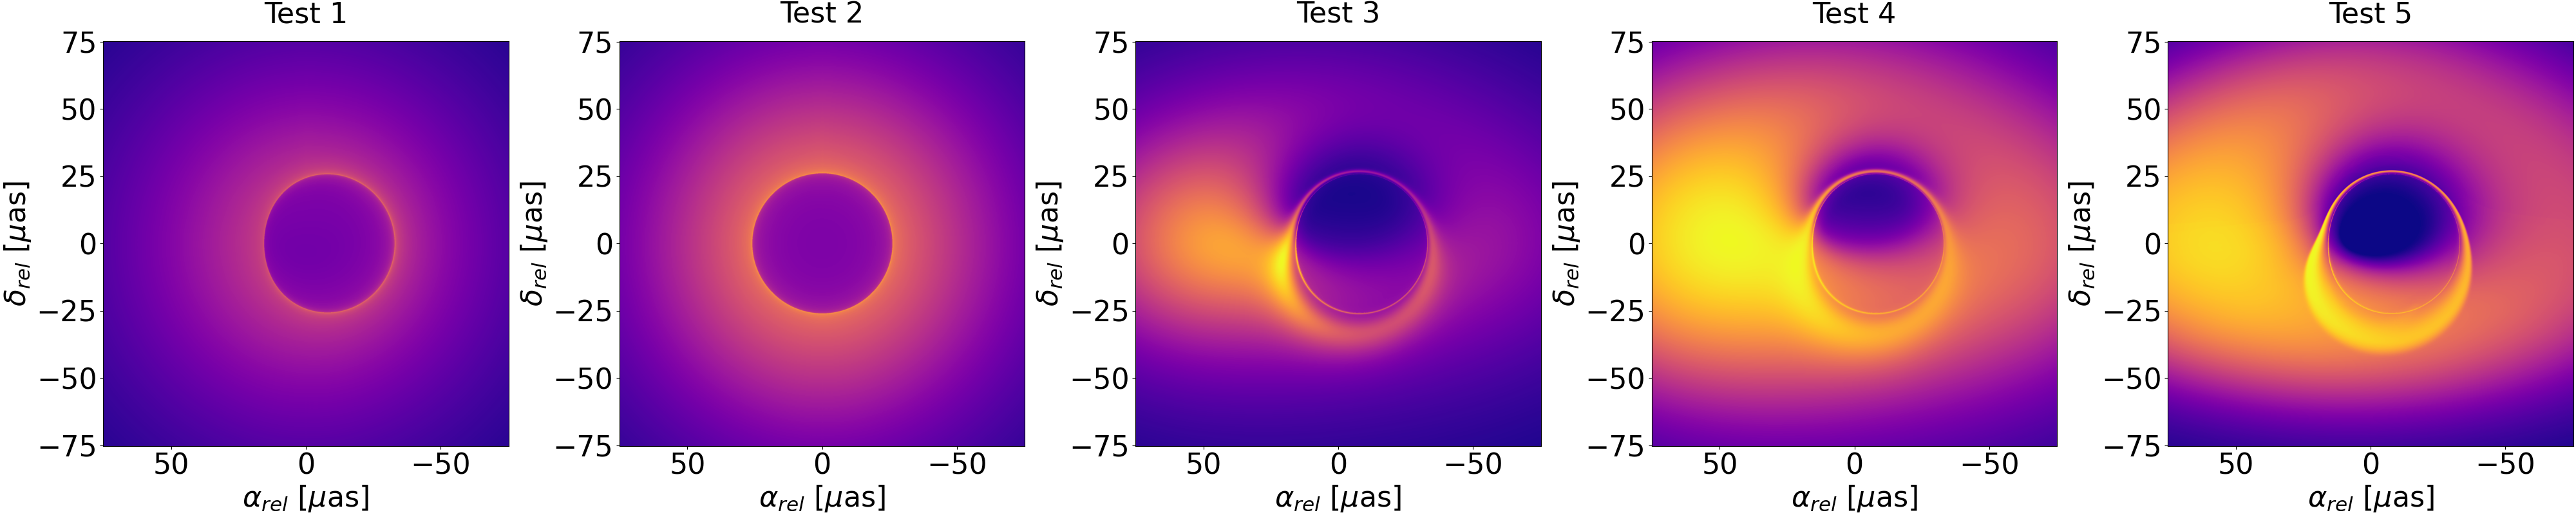
\includegraphics[scale = 0.15]{Verification_sims.png}

	\label{Verification_sims}
	\caption[Симулации за верификация на неполяризираният лъчист пренос]{\small Симулации за верификация на неполяризираният лъчист пренос, съответстващи на глава 5.2 от \cite{Gold2020}. Пълните потоци за всяка от петте симулации са дадени в таблица \ref{table:Sim_Verification_flux}. Поради голямата разлика в потоците, цветовата карта на всеки панел от тази фигура е нормирана на \emph{собственият} си максимум.} 
\end{figure}

\begin{table}[h!]
	\centering
	\begin{tabular}{c|c|c|c|c}
		\hline
		{Тест 1 [Jy]} & {Тест 2 [Jy]} & {Тест 3 [Jy]} & {Тест 4 [Jy]} & {Тест 5 [Jy]}
		\\\hline\hline
		1.6512 & 1.441 & 0.4445 & 0.2663 & 0.0252
		\\\hline\hline
	\end{tabular}
	\caption[Получени потоци от симулациите за верификация на неполяризираният лъчист пренос.]{\small Получени потоци от симулациите за верификация на неполяризираният лъчист пренос. За сравнение с други кодове виж \cite{Gold2020}, таблица 2.}
	\label{table:Sim_Verification_flux}
\end{table}
Виждаме, че Mjølnir изчислява потоци, които са в съгласие със седемте кода разгледани в \cite{Gold2020}. На базата на това сравнение сме правили изчисленията си в \cite{Deliyski2024} (глава 8).

\end{appendices}
